\documentclass[
  unicode,a4paper,10pt,
  % aspectratio=169,
  xcolor = {dvipsnames,svgnames},
  hyperref ={colorlinks=true,citecolor=Navy,linkcolor=NavyBlue,urlcolor=purple},
  ja=standard,lualatex
]{beamer}
\renewcommand{\baselinestretch}{1.4}

% ---fonts---
\PassOptionsToPackage{quiet}{fontspec}
\usefonttheme{serif}
\mathversion{bold}
\usepackage{luatexja-fontspec}
\setmainfont{TeX Gyre Termes}
\setmainjfont{Noto Sans CJK JP}
% \setmainjfont[BoldFont = HaranoAjiGothic-Regular]{HaranoAjiMincho}
% \setmainjfont[BoldFont = IPAGothic]{IPAMincho}
\setmathrm{Latin Modern Roman}
% \usepackage{newtxmath}

\usepackage{newunicodechar}
\newunicodechar{–}{-}

% ---refer `texdoc xcolor' at the command line---

% ---Display \subsubsection at the Index
% \setcounter{tocdepth}{3}

% ---Setting about the geometry of the document----
% \usepackage{a4wide}
% \pagestyle{empty}

% ---Physics and Math Packages---
\usepackage{amssymb,amsfonts,amsthm,mathtools}
\usepackage{physics,braket,bm,slashed}

% ---underline---
\usepackage[normalem]{ulem}

% ---cancel---
\usepackage{cancel}

% --- surround the texts or equations
\usepackage{fancybox,ascmac}

% ---settings of theorem environment---
\usepackage{amsthm}
\theoremstyle{definition}

% ---settings of proof environment---
\renewcommand{\proofname}{\textbf{証明}}
\renewcommand{\qedsymbol}{$\blacksquare$}

% ---Insert the figure (If insert the `draft' at the option, the process becomes faster.)---
\usepackage{graphicx}
% \usepackage{subcaption}

% ----Add a link to a text---
\usepackage{url,hyperref}
\usepackage{xcolor}

% ---Tikz---
\usepackage{tikz,pgf,pgfplots,circuitikz}
\pgfplotsset{compat=1.15}
\usetikzlibrary{intersections,arrows.meta,angles,calc,3d,decorations.pathmorphing,positioning}

% ---Add the section number to the equation, figure, and table number---
\makeatletter
   \renewcommand{\theequation}{\thesection.\arabic{equation}}
   \@addtoreset{equation}{section}
   
   \renewcommand{\thefigure}{\thesection.\arabic{figure}}
   \@addtoreset{figure}{section}
   
   \renewcommand{\thetable}{\thesection.\arabic{table}}
   \@addtoreset{table}{section}
\makeatother

% ---enumerate---
% \renewcommand{\labelenumi}{$\arabic{enumi}.$}
% \renewcommand{\labelenumii}{$(\arabic{enumii})$}

% ---beamer settings---
\usefonttheme{professionalfonts}
\usecolortheme{seahorse}
\setbeamercolor{structure}{fg=white}
\setbeamercolor{local structure}{fg=red}
\setbeamertemplate{itemize item}[ball]
\setbeamertemplate{enumerate item}[circle]
\setbeamercolor{bibliography entry author}{fg=black}
\setbeamercolor{bibliography item}{fg=black}
\setbeamercolor{alerted text}{fg=RoyalBlue}
\setbeamertemplate{frametitle continuation}{}
\setbeamertemplate{footline}[frame number]
\setbeamertemplate{navigation symbols}{} 
\setbeamersize{text margin left=10pt, text margin right=10pt}

% ---tcolorbox---
\usepackage{tcolorbox}
\tcbuselibrary{theorems}
\tcbuselibrary{raster}
\tcbuselibrary{skins}
\newtcolorbox{bluebox}[2][]{enhanced,
colframe=RoyalBlue!40!white,
colback=RoyalBlue!10!white,
coltitle=black,
drop fuzzy shadow, title={#2}
,#1}
\newtcolorbox{redbox}[2][]{enhanced,
colframe=DarkRed!40!white,
colback=DarkRed!10!white,
coltitle=black,
drop fuzzy shadow, title={#2}
,#1}

% ---tcolorbox---
\usepackage{tcolorbox}
\tcbuselibrary{raster,skins,breakable}
\newtcolorbox{graybox}[1][]{frame empty, colback=black!10!white, sharp corners}

% ---Ignore the Warnings---
\usepackage{silence}
\WarningFilter{latexfont}{Some font shapes}
\WarningFilter{latexfont}{Font shape}
\WarningFilter{latexfont}{Size substitutions}
\ExplSyntaxOn
\msg_redirect_name:nnn{hooks}{generic-deprecated}{none}
\ExplSyntaxOff

% ---Citation on the slides---
\newcommand*{\citefone}[2]{
  \begin{tikzpicture}[remember picture, overlay]
    \node[anchor=north east, align=left] at ($(current page.north east)-(0,0.0)$){
    {\tiny
      \cite{#1}
      #2
    }
    };
  \end{tikzpicture}

  \vspace*{-20pt}
}

\newcommand*{\citeftwo}[4]{
  \begin{tikzpicture}[remember picture, overlay]
    \node[anchor=north east, align=left] at ($(current page.north east)-(0,0.0)$){
    {\tiny
      \cite{#1}
      #2
    }
    \\[-2.4ex]
    {\tiny
      \cite{#3}
      #4
    }
    };
  \end{tikzpicture}

  \vspace*{-20pt}
}

\newcommand*{\citefthree}[6]{
  \begin{tikzpicture}[remember picture, overlay]
    \node[anchor=north east, align=left] at ($(current page.north east)-(0,0.0)$){
    {\tiny
      \cite{#1}
      #2
    }
    \\[-2.4ex]
    {\tiny
      \cite{#3}
      #4
    }
    \\[-2.4ex]
    {\tiny
      \cite{#5}
      #6
    }
    };
  \end{tikzpicture}

  \vspace*{-20pt}
}

\newcommand*{\citefonev}[3]{
  \begin{tikzpicture}[remember picture, overlay]
    \node[anchor=north east, align=left, text width=#3cm] at ($(current page.north east)-(0,0.0)$){
    {{\fontsize{5pt}{0pt}\selectfont
      \cite{#1}
      #2\par}
    }
    };
  \end{tikzpicture}

  \vspace*{-20pt}
}

\newcommand*{\citeftwov}[5]{
  \begin{tikzpicture}[remember picture, overlay]
    \node[anchor=north east, align=left, text width=#5cm] at ($(current page.north east)-(0,0.0)$){
    {{\fontsize{5pt}{0pt}\selectfont
      \cite{#1}
      #2\par}

      {\fontsize{5pt}{0pt}\selectfont
      \cite{#3}
      #4\par}
    }
    };
  \end{tikzpicture}

  \vspace*{-20pt}
}

\newcommand*{\citefthreev}[7]{
  \begin{tikzpicture}[remember picture, overlay]
    \node[anchor=north east, align=left, text width=#7cm] at ($(current page.north east)-(0,0.0)$){
    {{\fontsize{5pt}{0pt}\selectfont
    \cite{#1}
    #2\par}

    {\fontsize{5pt}{0pt}\selectfont
    \cite{#3}
    #4\par}

    {\fontsize{5pt}{0pt}\selectfont
    \cite{#5}
    #6\par}
    }
    };
  \end{tikzpicture}

  \vspace*{-20pt}
}


% ---Title---
\title{
  title
}
\author{
  author
}
\date{Last modified: \today}

\begin{document}

\nocite{Arkani-Hamed:2001uol}

\begin{frame}

  \setbeamertemplate{blocks}[rounded][shadow=true]
  \setbeamercolor{block body}{bg=LimeGreen!10!white, fg=black}
  \begin{block}{}
    \vspace*{5pt}

    \centering\Large
    Anomalies on orbifolds
    \\
    \normalsize
    Nima Arkani-Hamed, Andrew G. Cohen, Howard Georgi.
    \\
    \small
    \href{https://doi.org/10.1016/S0370-2693(01)00946-7}{Physics Letters B 516 (2001) 395–402},
    \href{https://doi.org/10.48550/arXiv.hep-th/0103135}{arxiv:hep-th/0103135}.

    \vspace*{5pt}
  \end{block}

  \begin{center}
    安倍研 M1 宮根一樹\\
    2024 5/7 (火)
  \end{center}
\end{frame}


\begin{frame}{読んだ動機}

  この春休み、\textcolor{Green}{QFT}やKK理論をメインに勉強した。

  \vspace*{5pt}
  
  くりこみ、有効作用、(非可換)ゲージ場の(経路積分)量子化など$\cdots\cdots$。

  \vspace*{5pt}
  \pause
  
  その中で、\textcolor{DarkOrange}{アノマリー}を勉強してみたいなと思いました。

  (教科書の写真を2つ)

\end{frame}


\begin{frame}

  一方で、この研究室でも高次元の理論のアノマリーは調べてみたかったけど、良く分かっていなかった部分もある模様。
  \begin{figure}[ht]
    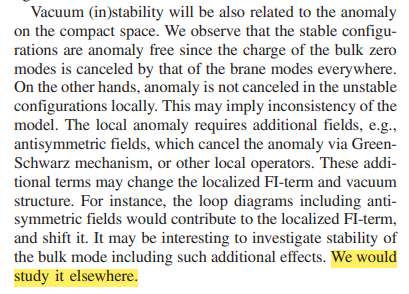
\includegraphics[width=0.7\textwidth]{fig/Abe2020vmv.png}
    \cite{Abe:2020vmv}
  \end{figure}

\end{frame}


\begin{frame}

  そこで、高次元のアノマリーに関連しているこの論文を読もうと思った。
  \begin{figure}[ht]
    \centering
    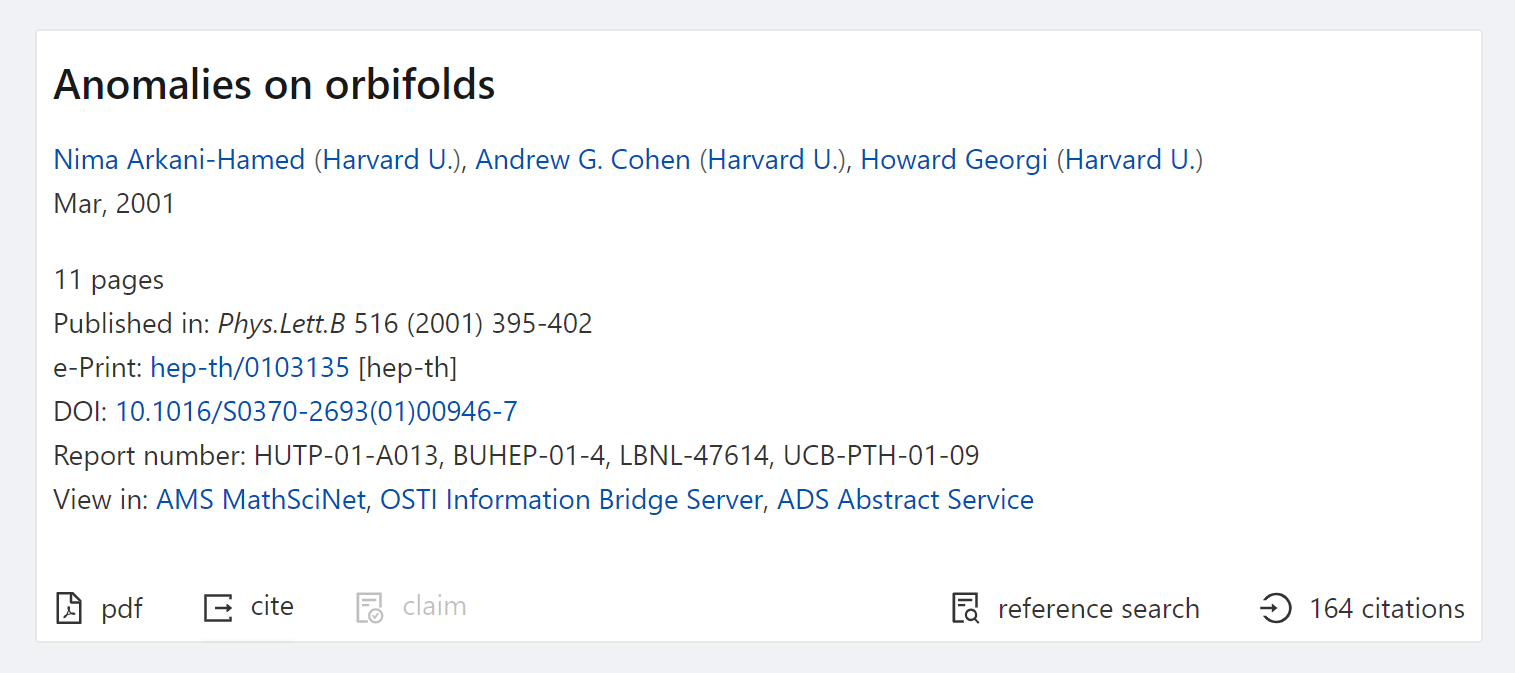
\includegraphics[width=0.7\textwidth]{fig/Arkani-Hamed2001uol.png}
  \end{figure}

\end{frame}


\section{イントロダクション}

\begin{frame}[plain]
  \huge \secname
\end{frame}

\subsection{アノマリー}

\begin{frame}{\subsecname}

  4次元の場合のカイラルアノマリーを確認する。

  \pause
  \vspace*{10pt}

  ゲージ場$A_{\mu}$と結合しているフェルミオン$\psi$を考える
  \begin{equation}
    \mathcal{L}
    =
    \bar{\psi}(i\slashed{\partial}-m)\psi
    +
    e\bar{\psi}\gamma^{\mu}\psi A_{\mu}
    \nonumber
  \end{equation}

  \vspace*{10pt}

  カイラル変換$\psi\rightarrow e^{i\gamma^{5}\alpha(x)}\psi$に対するネーターカレントの方程式は
  \begin{equation}
    \partial_{\mu}j^{\mu}_{5}
    =
    2im\bar{\psi}\gamma^{5}\psi
    ,\quad
    j^{\mu}_{5}
    =
    \bar{\psi}\gamma^{\mu}\gamma^{5}\psi
    \nonumber
  \end{equation}

\end{frame}



\begin{frame}

  しかし、この結果は古典論の結果

  \begin{equation}
    \partial_{\mu}
    (\bar{\psi}\gamma^{\mu}\gamma^{5}\psi)
    =
    2im\bar{\psi}\gamma^{5}\psi
    \nonumber
  \end{equation}

  \pause
  \vspace*{10pt}

  量子論の意味では、以下のファインマンダイアグラムの計算をすることと等価

  (ファインマンダイアグラムを2つほど)


\end{frame}


\begin{frame}  

  左側のダイアグラムの振幅を計算して位置基底に戻すと
  \begin{equation}
    \partial_{\mu}
    \ev*{\bar{\psi}\gamma^{\mu}\gamma^{5}\psi}
    =
    2im\ev*{\bar{\psi}\gamma^{5}\psi}
    +
    \textcolor{DarkGreen}{
      Q
    }
    ,\quad    
    \textcolor{DarkGreen}{
      Q
    }
    =
    \textcolor{DarkGreen}{
      \frac{e^2}{16\pi^2}\varepsilon^{\mu\nu\rho\sigma}\ev*{F_{\mu\nu}F_{\rho\sigma}}
    }
    \nonumber
  \end{equation}
  
  この余分な$\textcolor{DarkGreen}{Q}$は、ゲージ不変性を保って発散を正則化するときに生じる項

  \begin{center}
    この$\textcolor{DarkGreen}{Q}$を\textcolor{DarkRed}{カイラルアノマリー}という。    
  \end{center}  

  理論にアノマリーがあると、通常の量子論の定式化ができなくなることが知られている\cite{Fujikawa:2001b}。  (例えば、S行列のユニタリティーが保証できない。)

  \pause

  よって、
  \setbeamertemplate{blocks}[rounded][shadow=true]
  \setbeamercolor{block body}{bg=Goldenrod!10!white, fg=black}
  \begin{block}{}
    \centering
    アノマリーが相殺されるように理論を作りたい
  \end{block}  

\end{frame}


\subsection{Kaluza-Klein理論とアノマリー}

\begin{frame}{\subsecname}

  一方で、高次元の時空を考え、余剰空間に周期条件を与えること(コンパクト化)によって、4次元有効理論を作る方法があり、それをKaluza-Klein理論という。

  \vspace*{5pt}

  特に、今回は5次元の時空$x^{M}=(x^{0},x^{1},\cdots,x^{4})$を考え、$x^{4}$の方向に$x^{4}\sim x^{4}+2L$の周期境界条件を課してコンパクト化する。

  \pause
  \vspace*{10pt}

  \setbeamertemplate{blocks}[rounded][shadow=true]
  \setbeamercolor{block body}{bg=RoyalBlue!10!white, fg=black}
  \begin{block}{}
    \centering
    \textcolor{Green}{5次元の理論}でのアノマリー相殺
    \\
    と
    \\
    \textcolor{FireBrick}{4次元有効理論}でのアノマリー相殺
    \\
    の対応
  \end{block}
  を調べたい。

\end{frame}

\begin{frame}{オービフォールド$S^{1}/Z_{2}$}

  今回は、さらに\textcolor{Goldenrod}{オービフォールド}という境界条件を余剰空間に課す。
  
  \pause
  \vspace*{10pt}

  例えば、スカラー場の理論を考える
  \begin{equation}
    S
    =
    \int\dd^5 x\ 
    \left(  
      \frac{1}{2}\partial^{M}\Phi\partial_{M}\Phi
      -
      \frac{1}{2}m(x^{4})^2\Phi^2
    \right)
    \nonumber
  \end{equation}

  この理論に、$\Phi(x,x^{4})=\Phi(x,x^{4}+2L)$という境界条件に加えて
  \begin{equation}
    \Phi(x,x^{4})
    =
    \eta
    \Phi(x,-x^{4})
    \ ,\ 
    \eta=\pm 1
    \nonumber
  \end{equation}
  という境界条件を課す。  

\end{frame}

\begin{frame}
  \frametitle{}

  まずは、周期境界条件$\Phi(x,x^{4})=\Phi(x,x^{4}+2L)$から
  \begin{equation}
    \Phi(x,x^{4})
    =
    \sum_{n=-\infty}^{\infty}\phi_{n}(x) \exp \left[ i\frac{n\pi}{L}x^{4} \right]
    \nonumber
  \end{equation}
  とフーリエ展開できる。

  \vspace*{5pt}

  さらに、オービフォールドの境界条件$\Phi(x,x^{4})=-\Phi(x,-x^{4})$を課すと$\phi_{n}(x)+\phi_{-n}(x)=0$という条件になる

  \vspace*{5pt}

  この条件により、$n=0$のモード$\phi_{0}(x)$は消えることがわかる

  \pause
  \vspace*{5pt}

  \setbeamertemplate{blocks}[rounded][shadow=true]
  \setbeamercolor{block body}{bg=RoyalBlue!10!white, fg=black}
  \begin{block}{}
    \centering
    境界条件をうまく選べば、ゼロモードの場を消したり残したりできるため
    \\
    4次元の有効理論を作るときに嬉しい
  \end{block}
  ので、調べられている。

\end{frame}


\begin{frame}
  \frametitle{本論文の流れ・まとめ}

  

\end{frame}


\section{本論}

\begin{frame}[plain]
  \huge \secname
\end{frame}

\begin{frame}
  \frametitle{セットアップ}



\end{frame}


% --------------------------

\newcounter{Appendix}
\setcounter{Appendix}{\value{framenumber}}
\setcounter{section}{0}
\renewcommand{\thesubsection}{\Alph{subsection}}
\makeatletter
\renewcommand{\theequation}{\thesubsection.\arabic{equation}}
\@addtoreset{equation}{section}

\renewcommand{\thefigure}{\thesubsection.\arabic{figure}}
\@addtoreset{figure}{section}

\renewcommand{\thetable}{\thesubsection.\arabic{table}}
\@addtoreset{table}{section}
\makeatother

\section{付録}

\begin{frame}[plain]
  \frametitle{\ }
  \huge \secname
\end{frame}

\subsection{目次}

\begin{frame}[plain]{\thesubsection. \subsecname}
  \tableofcontents
\end{frame}


\subsection{4次元のカイラルアノマリーの計算}


\begin{frame}{\thesubsection. \subsecname}

  QEDのカイラルアノマリーを計算する。
  

\end{frame}

% --------------------------

\section{参考文献}
\begin{frame}[plain,allowframebreaks]{\secname}

  \scriptsize
  \beamertemplatetextbibitems
  \bibliographystyle{ytphys}
  \bibliography{ref}

  \nocite{Fujikawa:2001a}
  \nocite{Fujikawa:2001b}
  \nocite{Choi:2020dws}

\end{frame}

\setcounter{framenumber}{\value{Appendix}}
\end{document}
